\documentclass[../tech_report_1.tex]{subfiles}
\graphicspath{{img/}{../img/}}
\begin{document}

\part{Karcher Mean }

The Karcher mean is a geometric mean of various matrices and an extension
of the well known geometric mean of two matrices. It is also referred
to as the Riemannian geometric mean. In our investigation, we used
it as a way to compute the average distance between two points on
a hypersphere while obeying the curvature of the manifold. The process
is stated in Algorithm 1. In order to do this we must incorporate a
Logarithm map and Exponential map on the manifold. 




The Logarithm map is defined as a function that takes a point, $\rho_{2}$,
on the manifold and maps its projection vector, $\gamma$, on the
tangent plane at an origin point, $T_{p_{1}}$. 
\begin{equation}
\rho_{2}=Exp_{\rho_{1}}(\gamma)=cos(|\gamma|)\rho_{1}+sin(|\gamma|)\frac{\gamma}{|\gamma|}\label{eq:1}
\end{equation}
On the first iteration, $\rho_{1}$ is the origin point of the tangent
space.

The Exponential map can be thought of as the inverse function of the
Logarithm map. It is a function that takes in a vector on the tangent
plane at origin point and maps it on the hypersphere. As the difference
between the updating vectors on the tangent space begin to show little
change, it is thought as the optimal mean between the two points on
the manifold.
\begin{equation}
\gamma=Log_{\rho_{1}}(\rho_{2})=\tilde{\rho}\frac{cos^{-1}(\langle\rho_{1},\rho_{2}\rangle)}{\sqrt{\langle\tilde{\rho},\tilde{\rho}\rangle}}\label{eq:2}
\end{equation}
where $\tilde{\rho}=\rho_{2}-\langle\rho_{2},\rho_{1}\rangle\rho_{1}$.
Karcher mean, as we have mentioned before, is calculated in a way
to obey the curvature of the hypershere.


\section{Spherical mean}

Unlike the Karcher mean, the spherical mean does not go along the
curvature of the hypersphere. In the assignment step of this algorithm,
where we adjust the cluster centers, we find the mean by summing up
all the vectors in a cluster and normalizing it back onto the manifold.
\[
x_{l}=\frac{\sum_{i\in X_{l}}\rho_{i}}{||\sum_{i\in X_{l}}\rho_{i}||},l=1\dots K
\]
 where $X_{h}$ are the center of each $K$ number of clusters. This
is the normalized gravity center of the new cluster. 


\section{Our Implementation}

To find the best approach in calculating a cluster center, we put
Karcher mean and Spherical K-mean to the test. We tested them in five
types of situations in where the angles are either identical, orthogonal,
opposite, two random angles, or multiple random angles as shown in
Figure \ref{fig:Different-test-cases}. 

We found that Karcher mean and Spherical K-means produced the same
results as long as the step size for Karcher mean was set to one.
But both approaches failed in the case where the angles were opposite. 

\begin{figure}[ht]
\begin{centering}
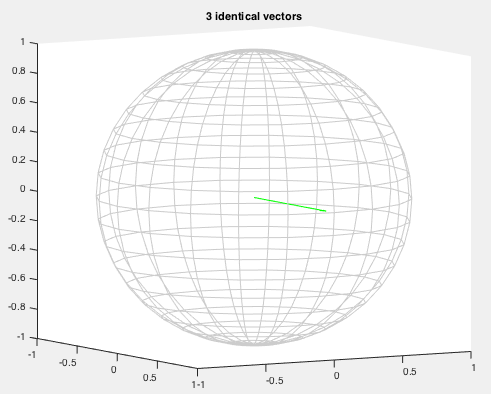
\includegraphics[width=2in]{fig1}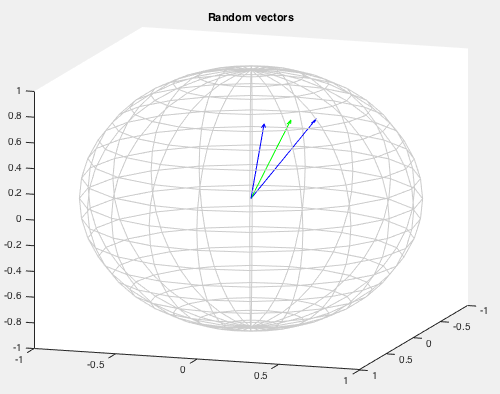
\includegraphics[width=2in]{fig2} 
\par\end{centering}

\begin{centering}
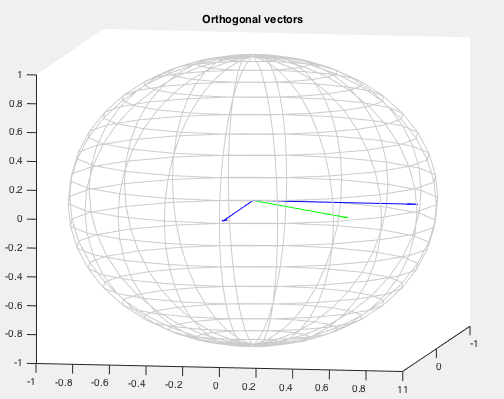
\includegraphics[width=2in]{fig3}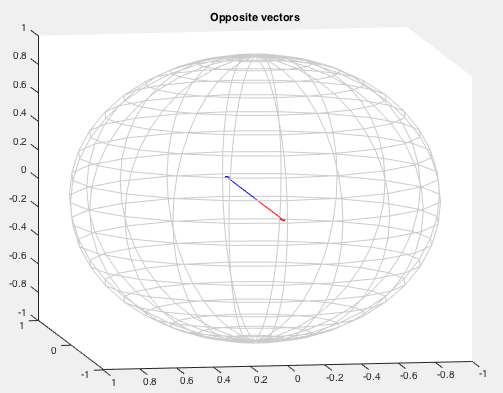
\includegraphics[width=2in]{fig4}
\par\end{centering}

\begin{centering}
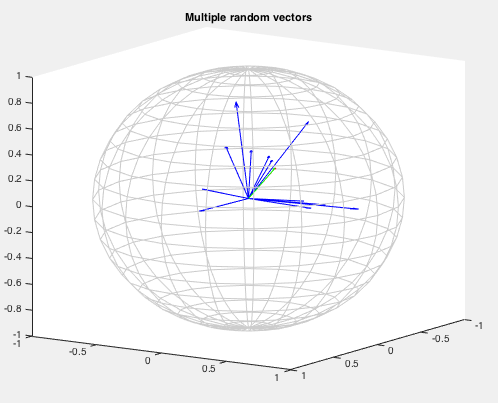
\includegraphics[width=2in]{fig5.png}
\par\end{centering}

\caption{Different test cases comparing accuracy of Karcher mean and Spherical
K-means.\label{fig:Different-test-cases}}


\end{figure}
\end{document}
